\section{Analysis of results}\label{sec:analysis-of-results}
This section presents an interpretation of data from the evaluations.

\subsection{Architecture and structure}\label{subsec:4-2-architecture-and-structure}
Support for architectural concepts in the representations was varied: some of them supported more concepts (Gaouar, XANUI, OpenUIDL) and some \textendash\ less (Quid, Khan, Soude).
This might have been caused by different goals that these representations have.
For example, Quid is a minimal language and a browser tool for prototyping Web components \textendash\ it is therefore understandable that it does not incorporate a concept of an application.

Modularization was the only concept supported by all representations.
Additionally, judging by the results, the concept of a view is more important than the concept of an application \textendash\ it usually seems enough to be able to connect views with one another.
Dialogs (\textbf{A3}) and third-party components (\textbf{A6}) were not widely supported \textendash\ the former was only supported by a single representation (Verhaeghe), and the latter \textendash\ by two (OpenUIDL, XANUI).

\subsection{Logic and behavior}\label{subsec:4-2-logic-and-behavior}
Support for specifying the behavior of UI in the representations ranged from low to moderate \textendash\ three representations scored around 20--30\%, two \textendash\ around 50\% and XANUI achieved the maximum score of 66\%.
Most representations allowed for handling events and declaring methods attached to UI elements (\textbf{B1}, \textbf{B3}).
However, there was less support specifying the details of implementation of these handlers (\textbf{B4}, B8.1, \textbf{B10}, \textbf{B11}).
Sets of predefined events (\textbf{B2}) also varied in their scope from minimal (XANUI, Soude, Quid, Gaouar) to comprehensive (Verhaeghe, OpenUIDL).

Only one representation (XANUI) explicitly supported data validation (\textbf{B5}).
More were able to integrate with code outside the UI layer, either by calling some services (\textbf{B6}) or directly embedding scripts (\textbf{B7}).
Support for custom components (\textbf{B12}) was relatively rare \textendash\ only three representations meaningfully implemented this feature (XANUI, OpenUIDL, Quid).
Support for content as input (in OpenUIDL) and component methods (provided in Quid) was even rarer.

Khan et al.\ explicitly stated that their representation does not describe behavior \textendash\ it is meant to be implemented manually.
Although Verhaeghe et al.\ successfully used their description to migrate both the content and the logic of UIs, this success does not seem to translate to modelling on its own.
It might be so, because their behavior metamodel is based on a model of the abstract syntax tree (AST) that is used for modelling code of applications;
thus, the metamodel does not introduce any new concepts specific to the behavior of UI\@.

Quid allows for handling events, as well as an explicit definition of handlers; its capabilities are nevertheless limited in other areas.
Gaouar et al.\ also allow for defining handlers; on one hand, it is even possible for them to call external services, on the other \textendash\ they are rather limited in terms of control structures and operators.

Soude and Koussonda also allow for specifying handlers (at least for input components) and using external (REST) services.
Additionally, they support a wide range of expression operators and data types.
OpenUIDL has moderate capabilities of describing behavior;
its strongest points are comprehensive support for custom components and a wider set of predefined events.
The representation attempts to model component state and its changes, however, at the moment of evaluation, the functionality is in its early stage.
XANUI is the most expressive in this area, as it is an annotation language \textendash\ it is embedded into an implementation language which allows it to take advantage of its expressiveness.
However, the representation also provides a few constructions on its own (e.g.\ handlers and data validation).

\subsection{Component support}\label{subsec:4-2-component-support}
Support for predefined components in the chosen representations ranged from low to medium.
The least supported category were complex output components (\textbf{C3}) and specialized containers (\textbf{C1}) \textendash\ such a result is relatively understandable, as supporting additional types of components requires effort on the part of maintainers.
Interaction components (\textbf{C6}) and simple output components (\textbf{C2}) were moderately supported;
so were input components (\textbf{C4}), although usually their implementation lacked customization abilities (\textbf{C5}).

There does not seem to be any technical constraint that would explain the more or less limited set of components offered by the representations \textendash\ the results seem to be motivated by a subjective judgement of authors.
To be able to support them, maintainers would simply need to define them in the model and define a transformation rule that would include them in the final code;
that is exactly the approach Verhaeghe et al.\ recommend to users of their representation if the predefined set does not satisfy their needs.
The only exception here could be XANUI \textendash\ the relative lack of support for predefined components might also be explained by its relationship to the final UI code.

\subsection{Appearance}\label{subsec:4-2-appearance}
Support for describing appearance of the final UI was the most varied from all sections: some representations did not incorporate that aspect at all (Soude), while some had comprehensive support (OpenUIDL).

Most languages supported a linear layout (D1.1), as it can be used on its own to implement most of the layouts;
some also specified an additional one, e.g.\ a flex layout (D1.2), or a relative layout (D1.4).
A few languages (Gaouar, Khan, OpenUIDL) supported responsive layouts through media queries.

There was very varied support for sizing (\textbf{D3}) and positioning (\textbf{D5}) \textendash\ some representations provided most or all methods, and some none.
Only OpenUIDL provided a relatively wide set of sizing units (\textbf{D4});
most representations limited themselves to pixels (D4.1) and percentages (D4.4).

Regarding other style properties (\textbf{D6}, \textbf{D7}), support was either comprehensive (Khan, OpenUIDL) or nonexistent (Verhaeghe).
Extended capabilities for describing the appearance through CSS were only provided in two representations (Khan, OpenUIDL).

Some representations (Quid, Soude) dismiss the area of appearance of applications;
others model it with greater or smaller accuracy.
XANUI \textendash\ again \textendash\ does not include too much information about appearance, as this concern might be addressed outside the representation (e.g.\ through CSS).
Capabilities of OpenUIDL are definitely the most extensive of all representations.
Appearance is also the section where the representation achieves its highest score;
it scored most or all points on almost all criteria except layout capabilities.
The reason for this might be because the language is intended to model Web applications, where layouts other than linear or flex are not useful.

\subsection{General results}\label{subsec:general-results}

Figure~\ref{fig:4-2-results-per-section} visualizes the results for each section of evaluation.
As mentioned in previous subsections: representations have varied support for different areas.
Architectural concepts are the most supported, although this support is not as common as one could expect.
Most languages have little support for specifying logic and behavior and relatively narrow sets of predefined components.
Support for appearance lies on two extremes \textendash\ it is either implemented thoroughly or not present at all.

Figures~\ref{fig:4-2-results-per-representation} and~\ref{fig:4-2-results-total} present the results for each representation (grouped per section and overall, respectively).
One can see that although the representations sometimes have quite good support for certain UI areas, none of them scores consistently well.
Quid is the least expressive language from the set;
it has some basic support for logic of components, but cannot handle complexity in other areas.

Two next representations with the lowest scores (Khan, Soude and Koussonda) have some areas with strong support, as well as areas that were entirely ignored.
XANUI has strong support for architecture and logic, but very little support for components and appearance.
As pointed out earlier \textendash\ this notation might actually not need to support these concepts explicitly and use capabilities of the platform of the final UI.

Verhaeghe and Gaouar provide representations that are a little more balanced, but still do not excel in any particular area.
OpenUIDL is the most expressive of all representations, providing strong architectural support and good capabilities for customizing the appearance.
Its set of predefined is satisfactory and can be sufficient for a lot, but not a majority of use cases.
When it comes to behavior, its capabilities could be considered subpar \textendash\ it does not yet allow to fully customize it, although it already has the necessary framework to do so.

\begin{figure}
    \centering
    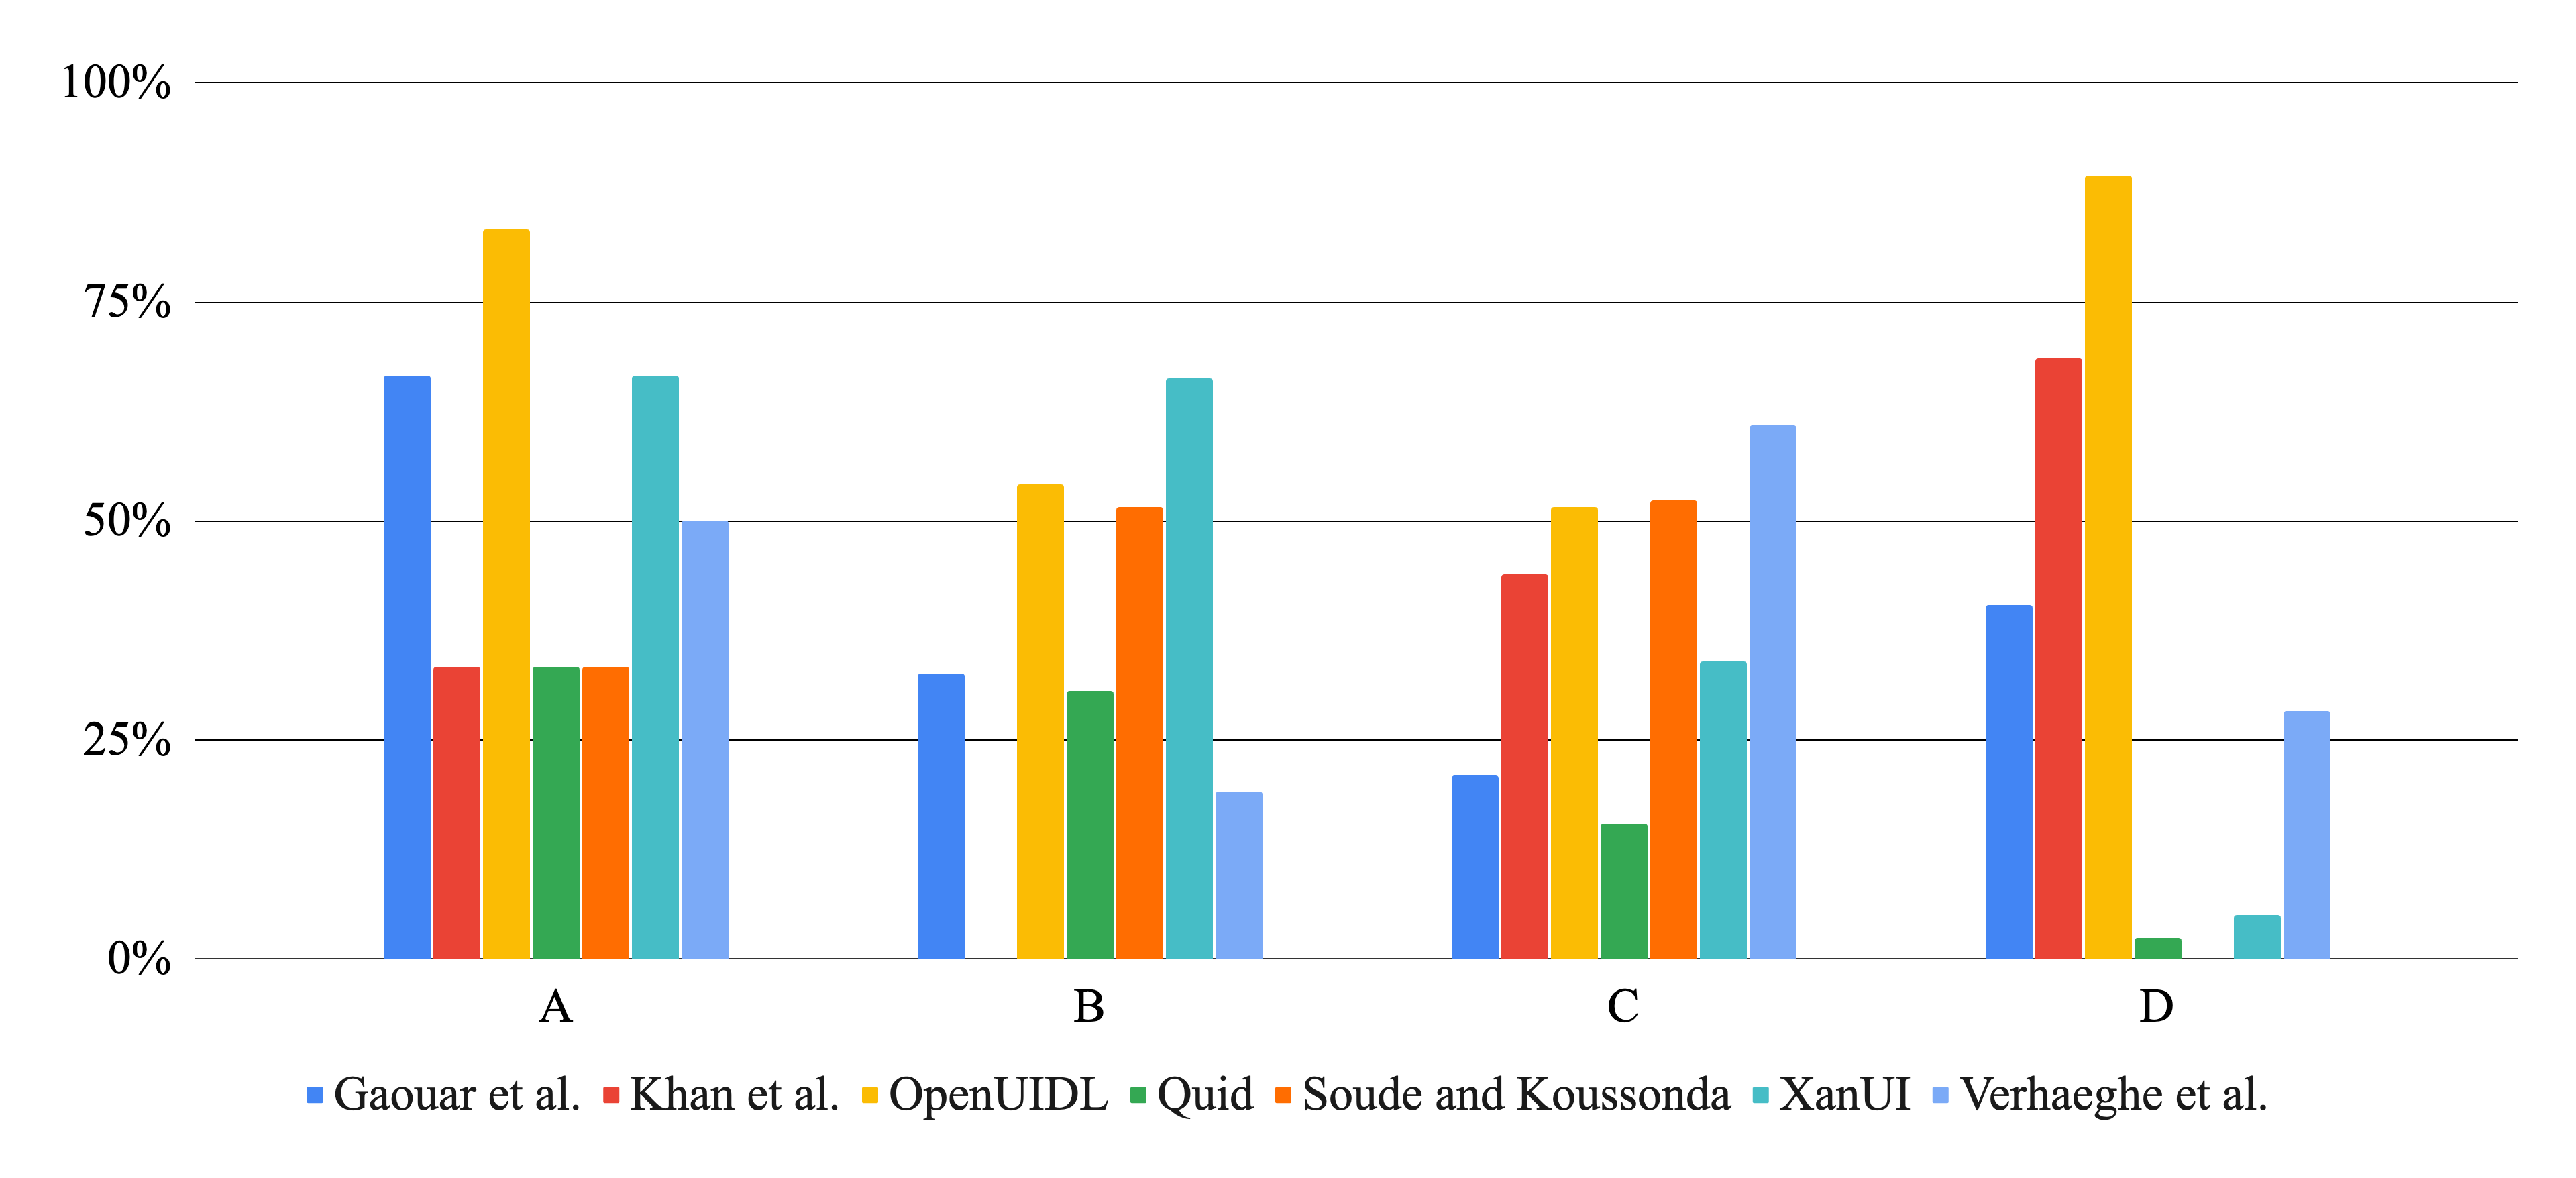
\includegraphics[width=\textwidth]{4-results-and-discussion/results-per-section}
    \caption{Results of the evaluation, presented per section}
    \label{fig:4-2-results-per-section}
\end{figure}

\begin{figure}
    \centering
    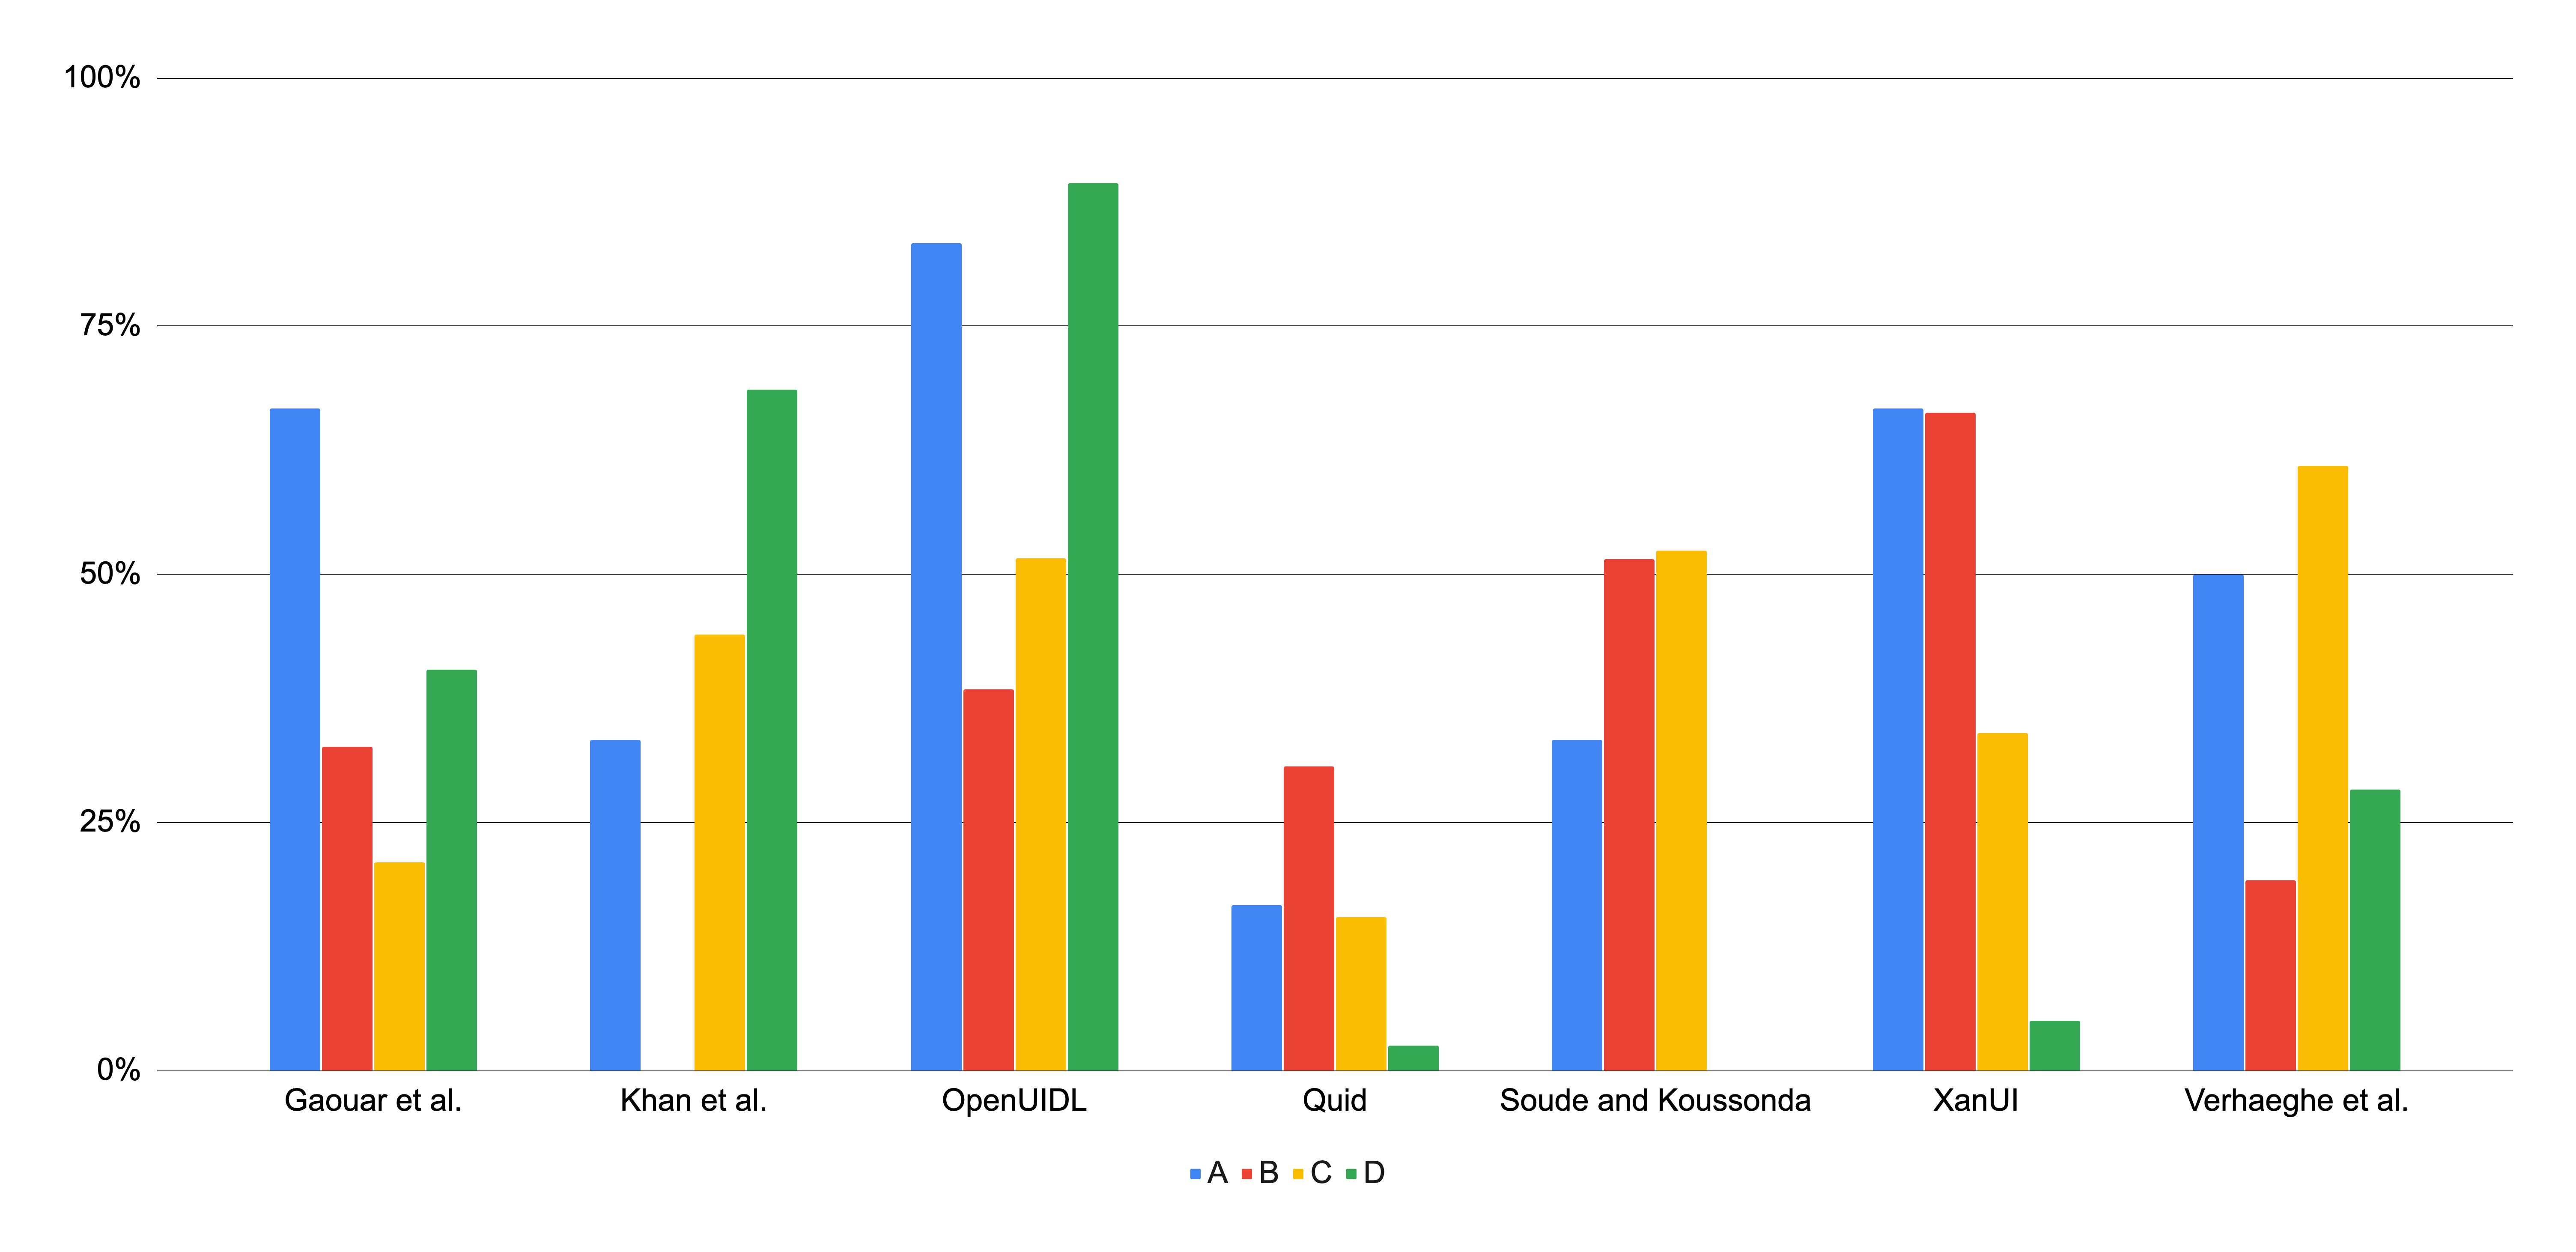
\includegraphics[width=\textwidth]{4-results-and-discussion/results-per-representation}
    \caption{Results of the evaluation, presented per representation}
    \label{fig:4-2-results-per-representation}
\end{figure}

\begin{figure}
    \centering
    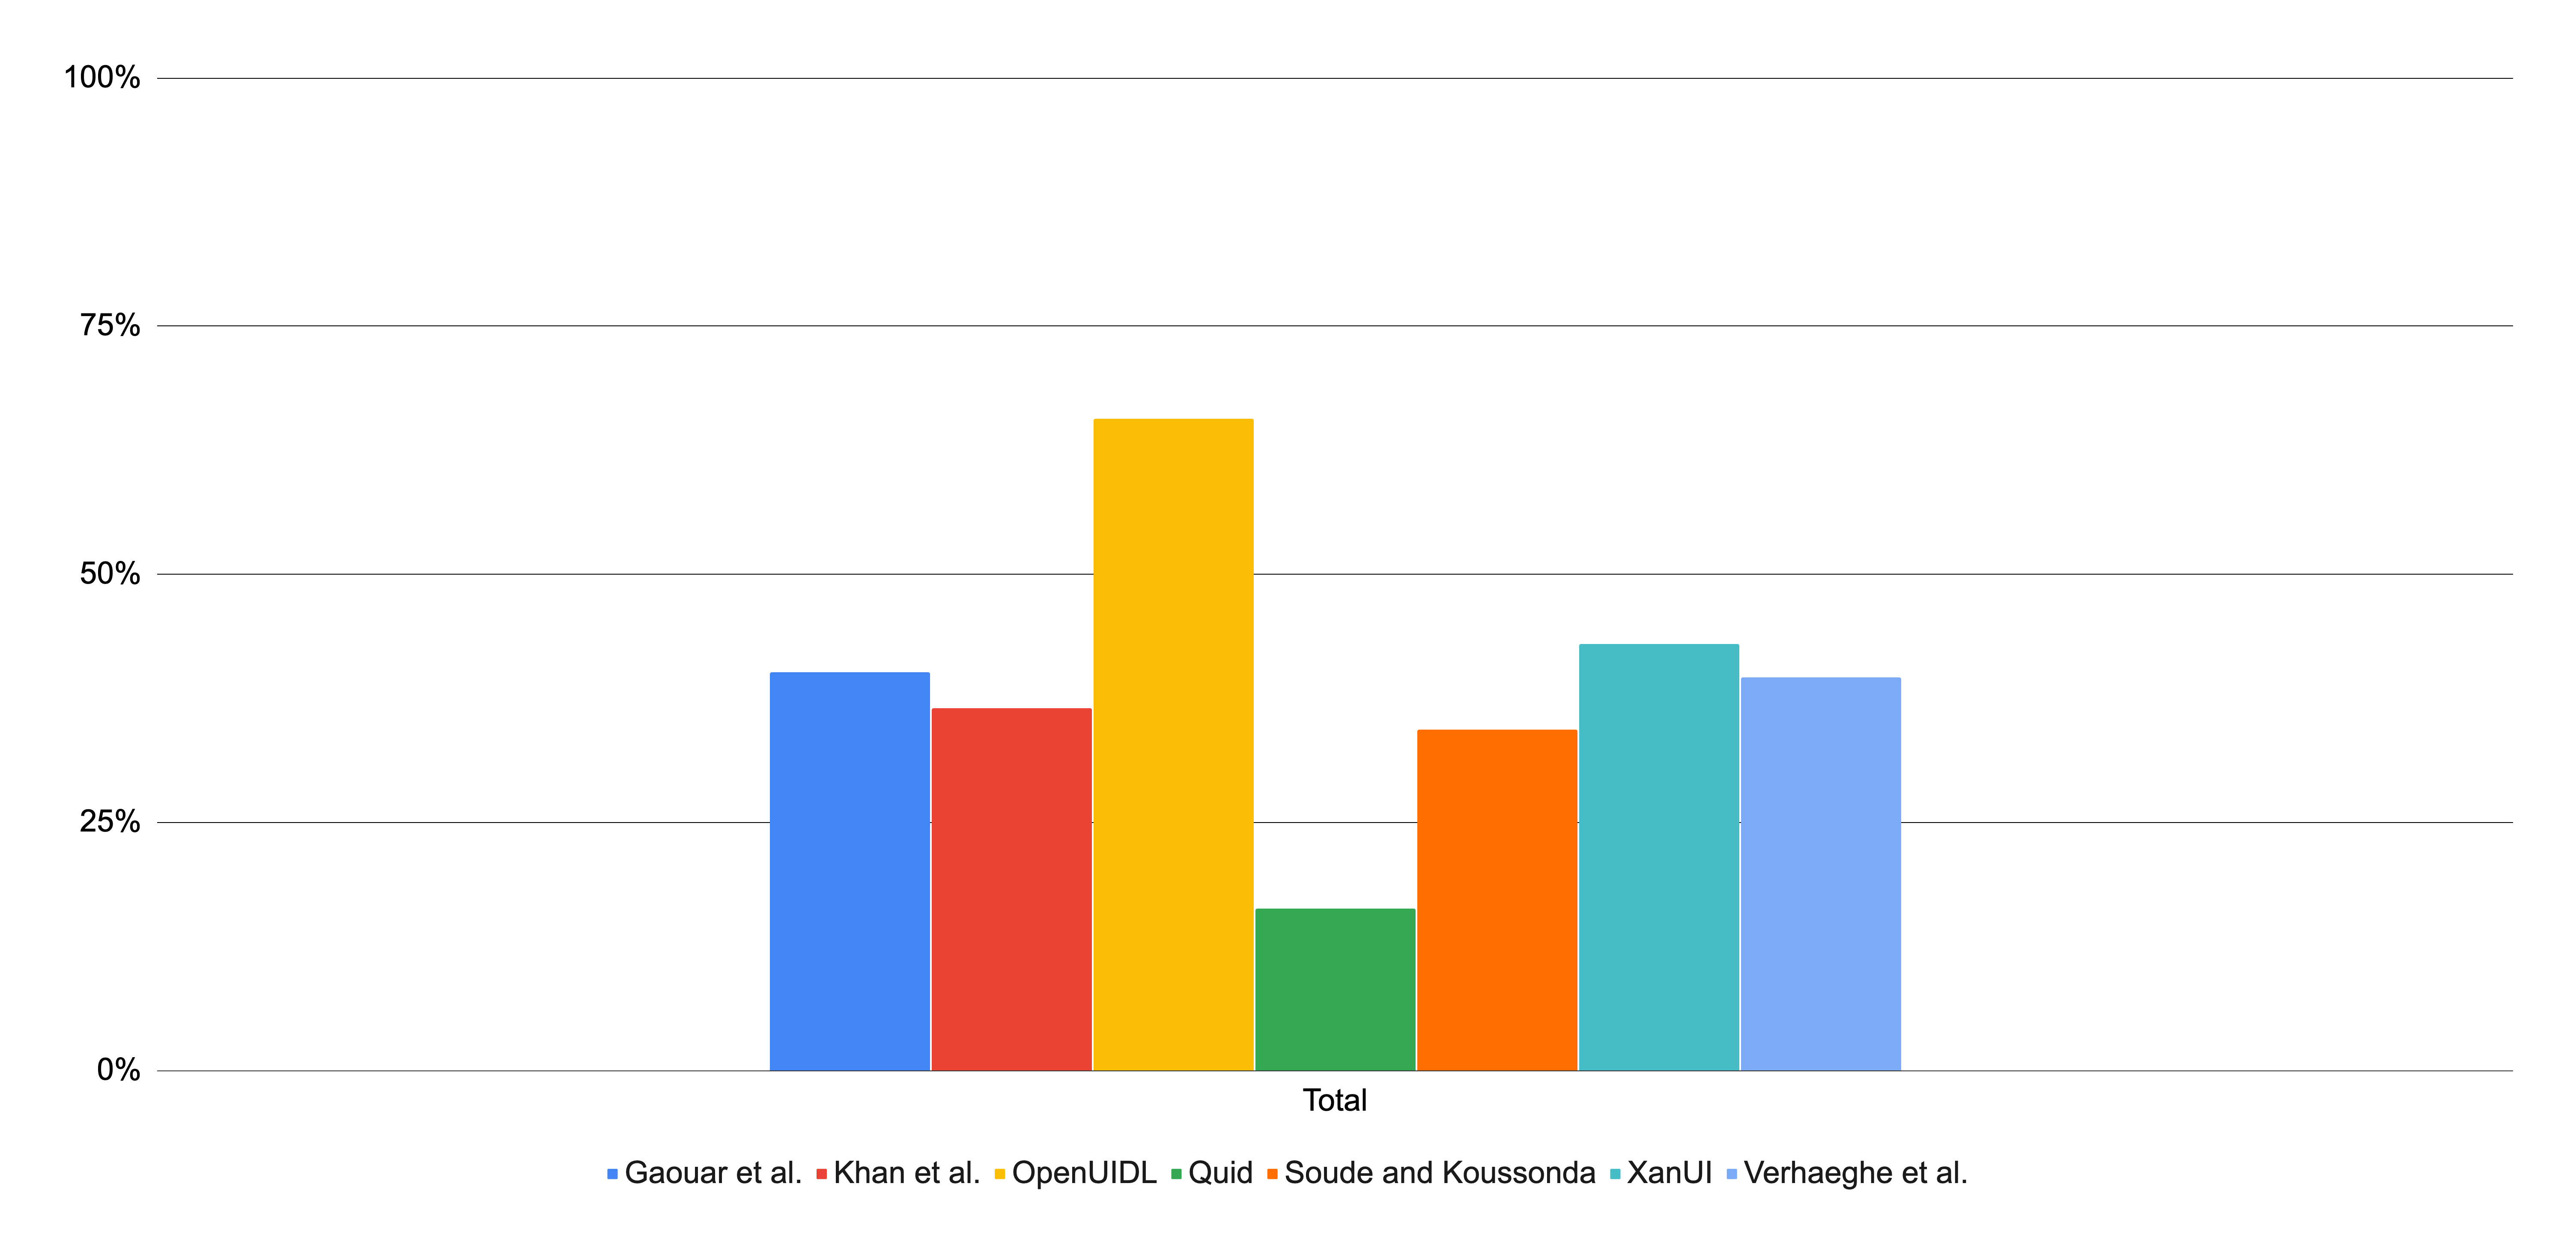
\includegraphics[width=\textwidth]{4-results-and-discussion/results-total}
    \caption{Overall results of the evaluation}
    \label{fig:4-2-results-total}
\end{figure}

\subsection{Case study}\label{subsec:case-study}
The results of the case study confirmed the findings from the theoretical evaluation, as selected representations scored similarly in both (Quid: 13\% in the case study, 20\% in the evaluation; OpenUIDL: 69\% in the case study, 70\% in the evaluation).
Figure~\ref{fig:4-2-board-view} presents the result of implementing the board view in both representations.

Quid, as evidenced both by the evaluation and the screenshot in figure~\ref{fig:4-2-quid-board-view}, could not be used to accurately reproduce the designed interface.
It was only possible to group data within a component and display it using either a horizontal or vertical layout; providing data to components or modifying their state did not work.
The representation also did not have any option to customize the appearance of components; even the set of provided components was also very narrow.

With OpenUIDL it was possible to create quite a faithful replication of an original design in terms of appearance (presented in figure~\ref{fig:4-2-openuidl-board-view}) \textendash\ this was thanks to the language's broad support for appearance properties.
It was also possible to implement a dropdown menu and prototype navigation between views.
As described previously \textendash\ although the representation allows for defining some simple state, event handlers, or component properties, it was not possible to implement any meaningful logic with these means.

\begin{figure}
    \centering
    \begin{subfigure}[m]{0.5\textwidth}
        \centering
        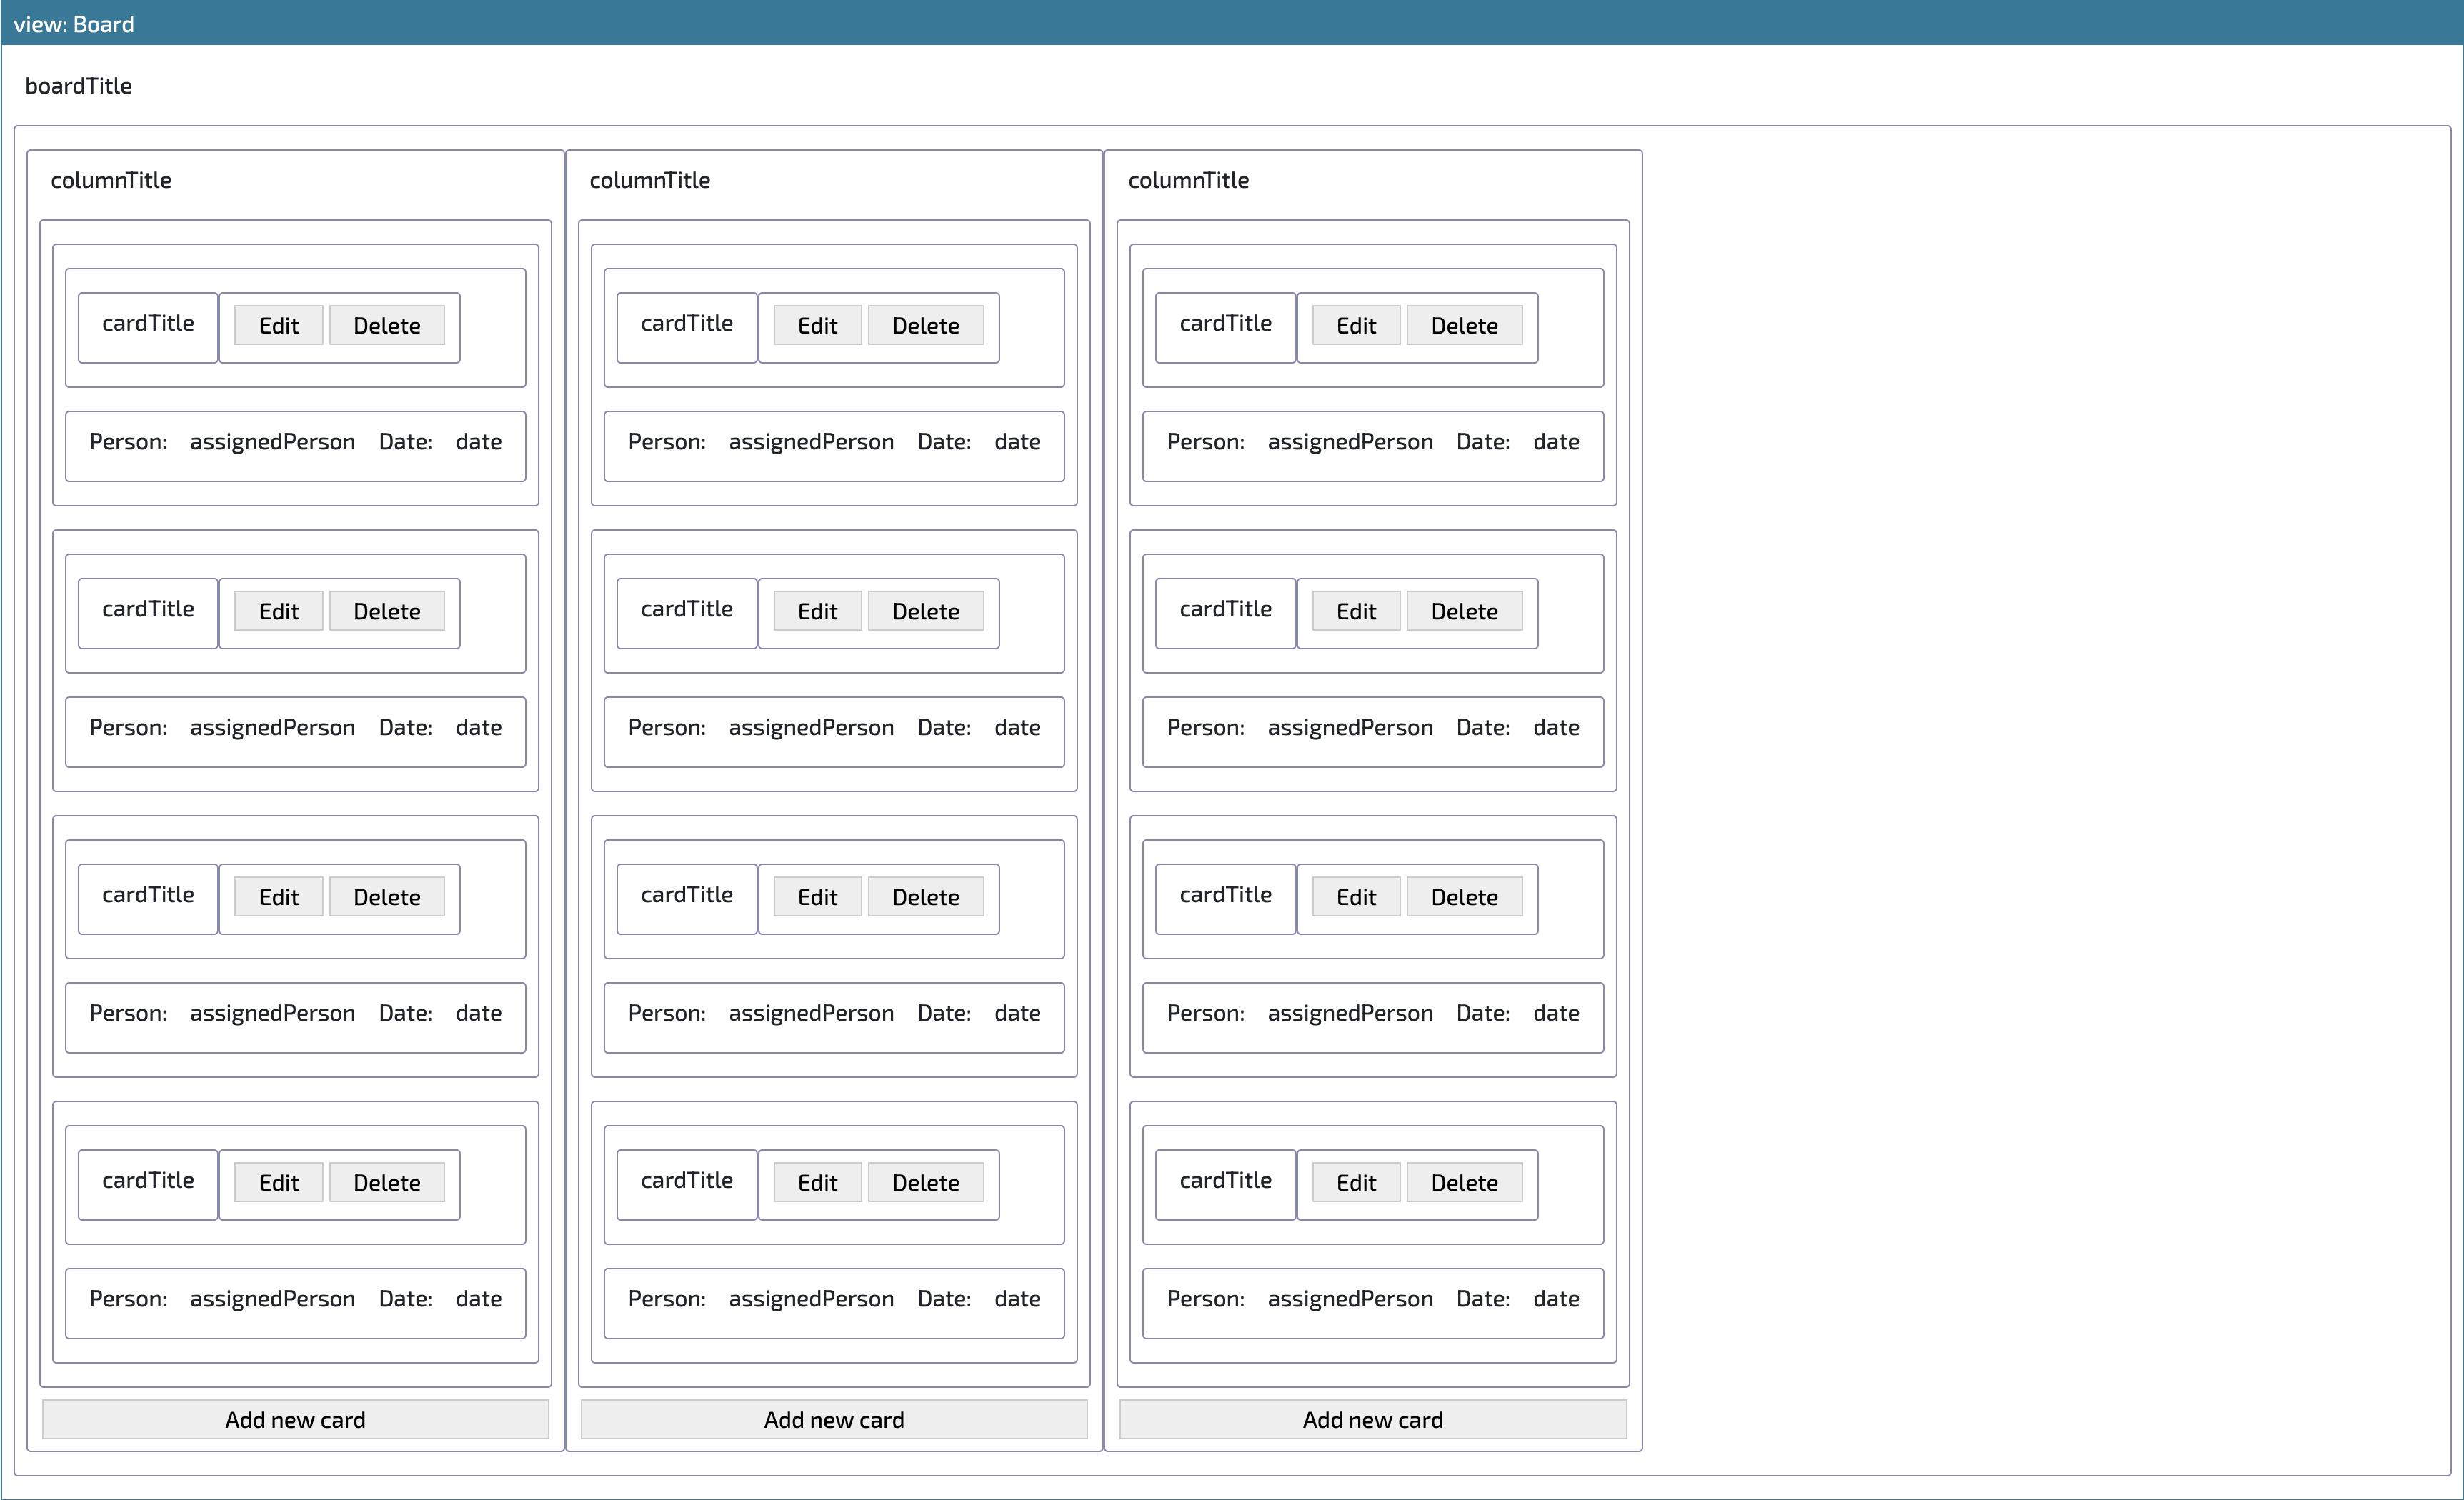
\includegraphics[height=0.2\textheight]{./4-results-and-discussion/quid-board-view}
        \caption{Board view implemented in Quid}
        \label{fig:4-2-quid-board-view}
    \end{subfigure}
    \hfill
    \begin{subfigure}[m]{0.35\textwidth}
        \centering
        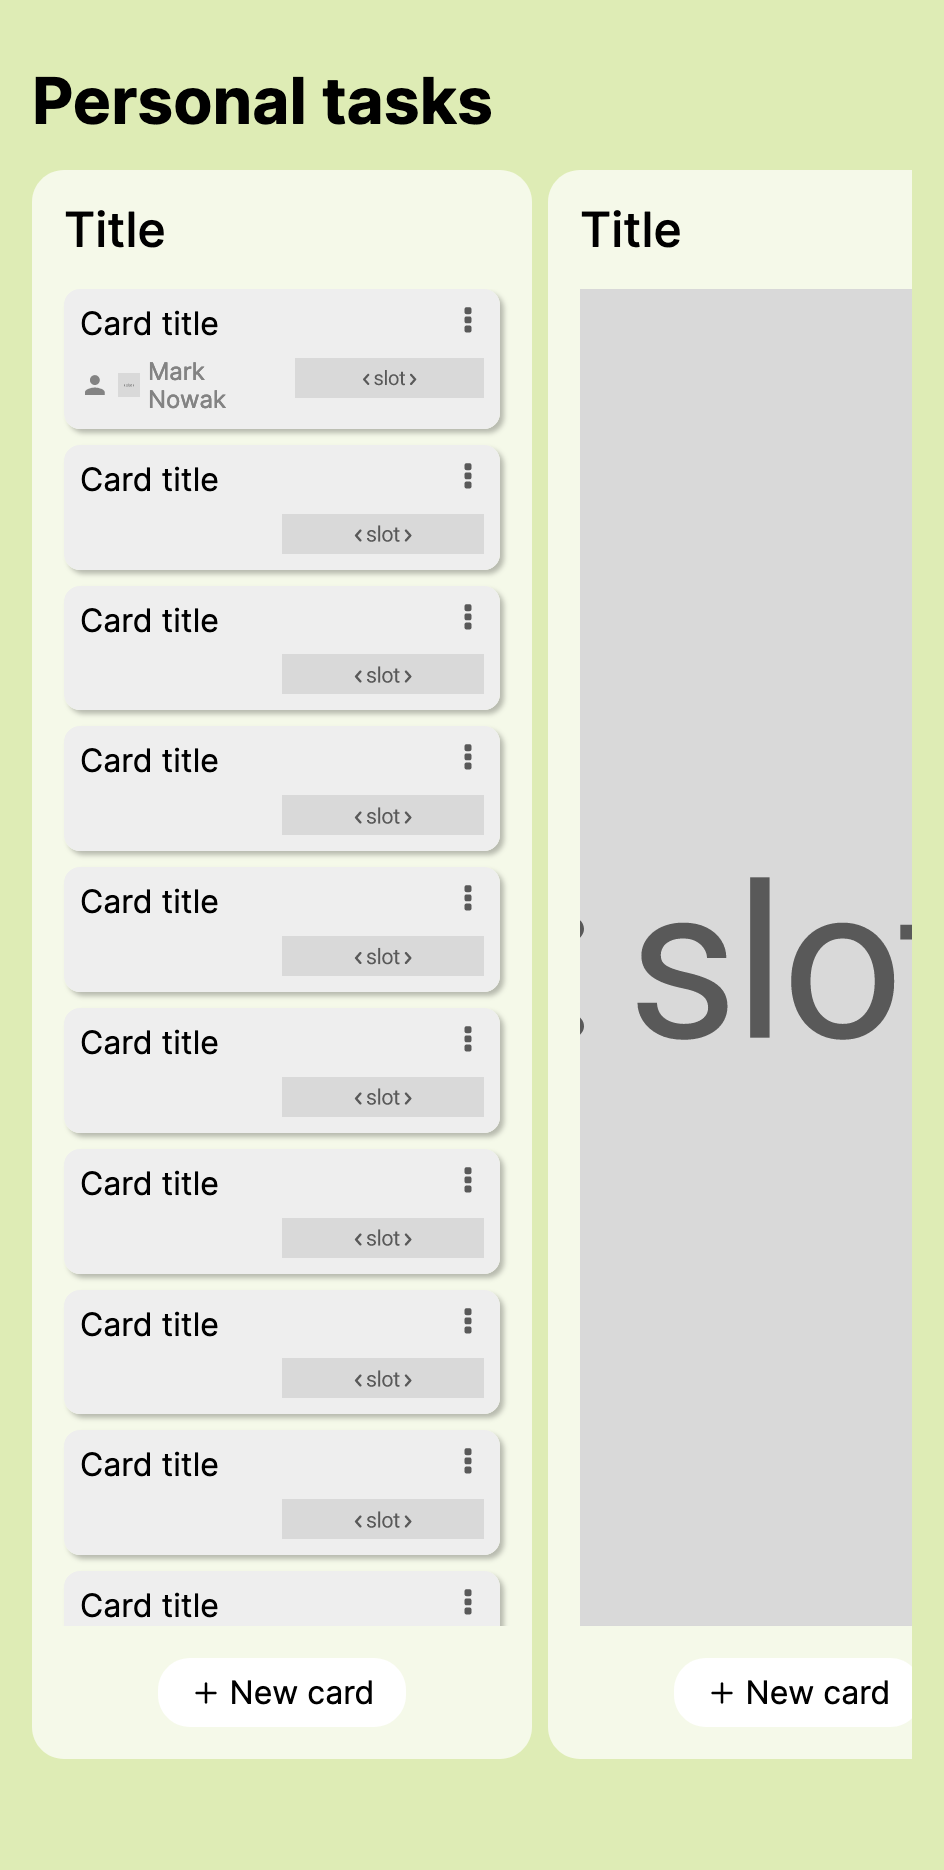
\includegraphics[height=0.3\textheight]{./4-results-and-discussion/openuidl-board-view}
        \caption{Board view implemented in OpenUIDL}
        \label{fig:4-2-openuidl-board-view}
    \end{subfigure}
    \caption{Implementations of the board view from the case study}
    \label{fig:4-2-board-view}
\end{figure}

\subsection{Results of the qualitative evaluation}\label{subsec:results-of-the-qualitative-evaluation}
Both Quid and OpenUIDL are available through online editors provided by their authors.
This can be considered useful, as the application is readily available on any computer with a modern Web browser.
One drawback of Web editors could be offline unavailability;
however, it could be mitigated with relatively little effort by turning the editors into progressive web apps~\furl{https://developer.mozilla.org/en-US/docs/Web/Progressive_web_apps}.

The two editors take two slightly different approaches to working with the underlying representations in different ways.
In Quid, the user edits the description directly and can immediately see the preview of the current view or component (as presented in figure~\ref{fig:4-2-quid-editor}).
On the other hand, OpenUIDL does not require that users write code and instead uses the what-you-see-is-what-you-get technique; authors of the representations provide a UI for designing the prototypes (figure~\ref{fig:4-2-openuidl-editor}).
UI is created by selecting elements from a list and dropping them onto an area which visualizes how a view or a component is going to look like.
OpenUIDL allows for previewing the code of the application in a final technology (e.g.\ React, Angular), but does not let users view or manipulate the underlying representation directly.
There is a possibility to also obtain a live preview of components and projects in a separate website~\furl{repl.teleporthq.io}, but it is not integrated with the other editor.
Hiding the representation is understandable, given the complexity of said representations \textendash\ Quid is a much simpler language than OpenUIDL, which makes it much more suitable for manual editing.
Nevertheless, such a restriction can hinder development and troubleshooting activities for more advanced users.

\begin{figure}
    \centering
    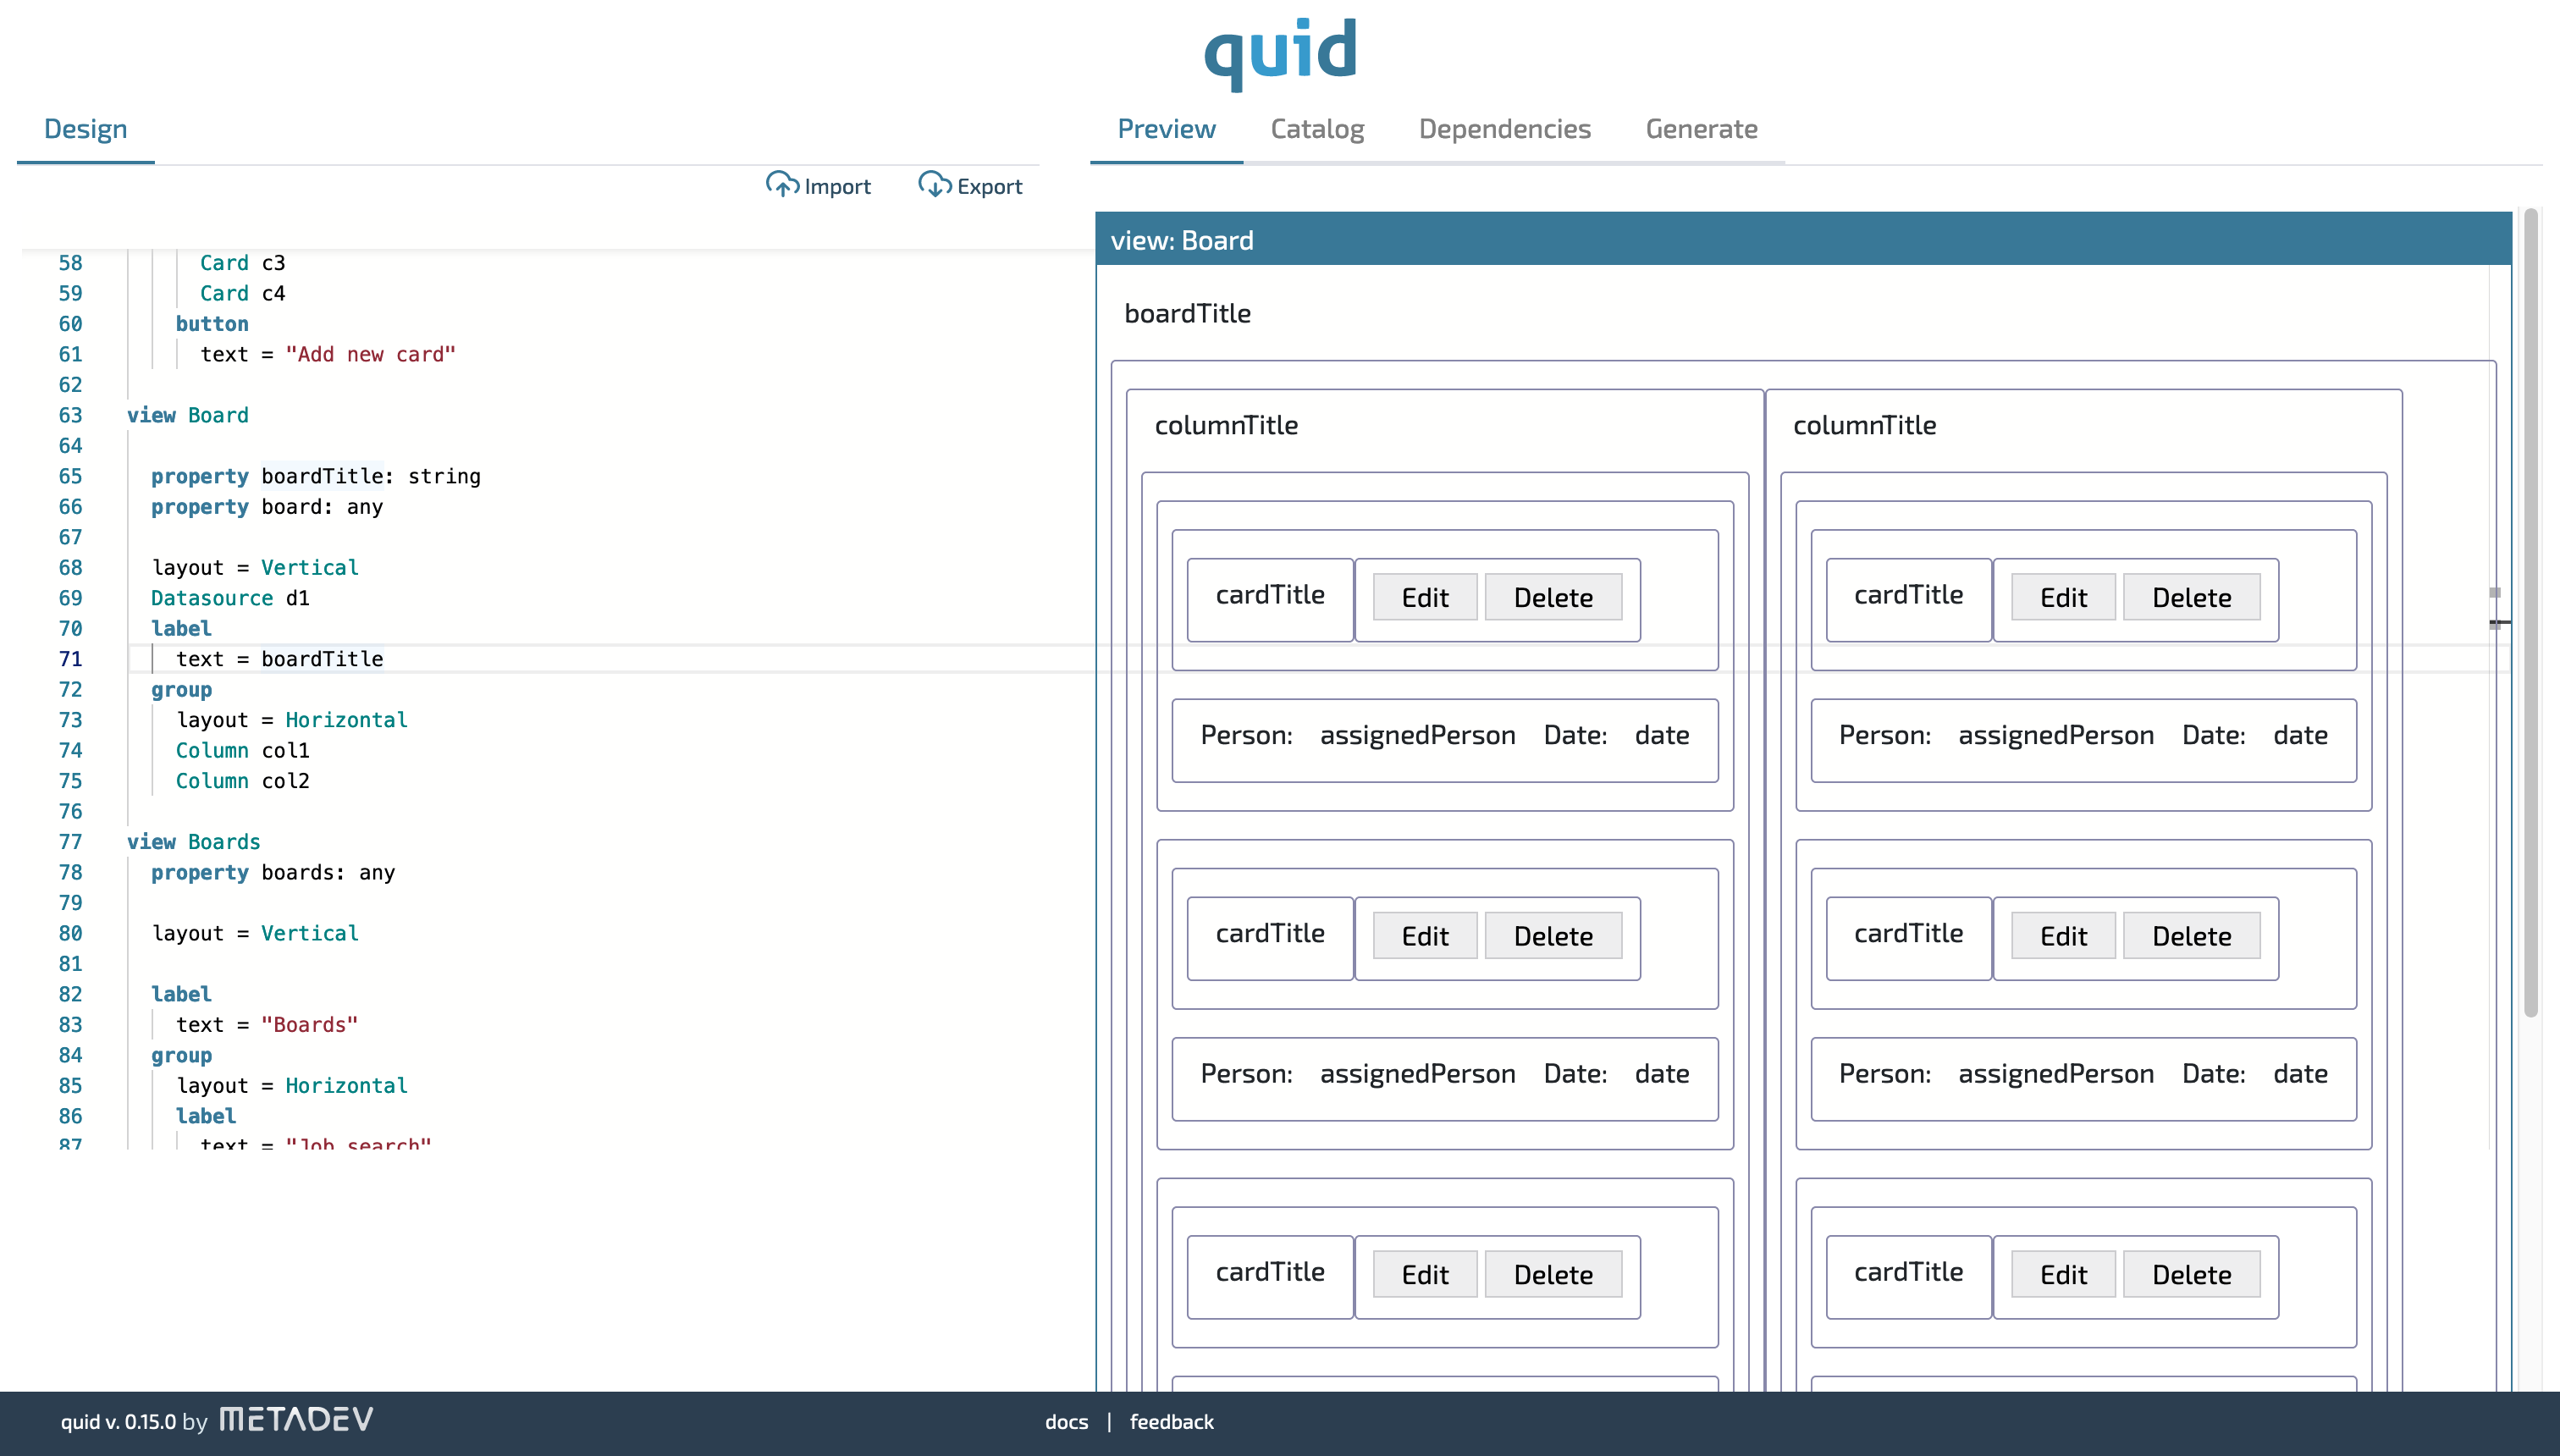
\includegraphics[width=\textwidth]{4-results-and-discussion/quid-editor}
    \caption{Screenshot of the Quid editor}
    \label{fig:4-2-quid-editor}
\end{figure}

\begin{figure}
    \centering
    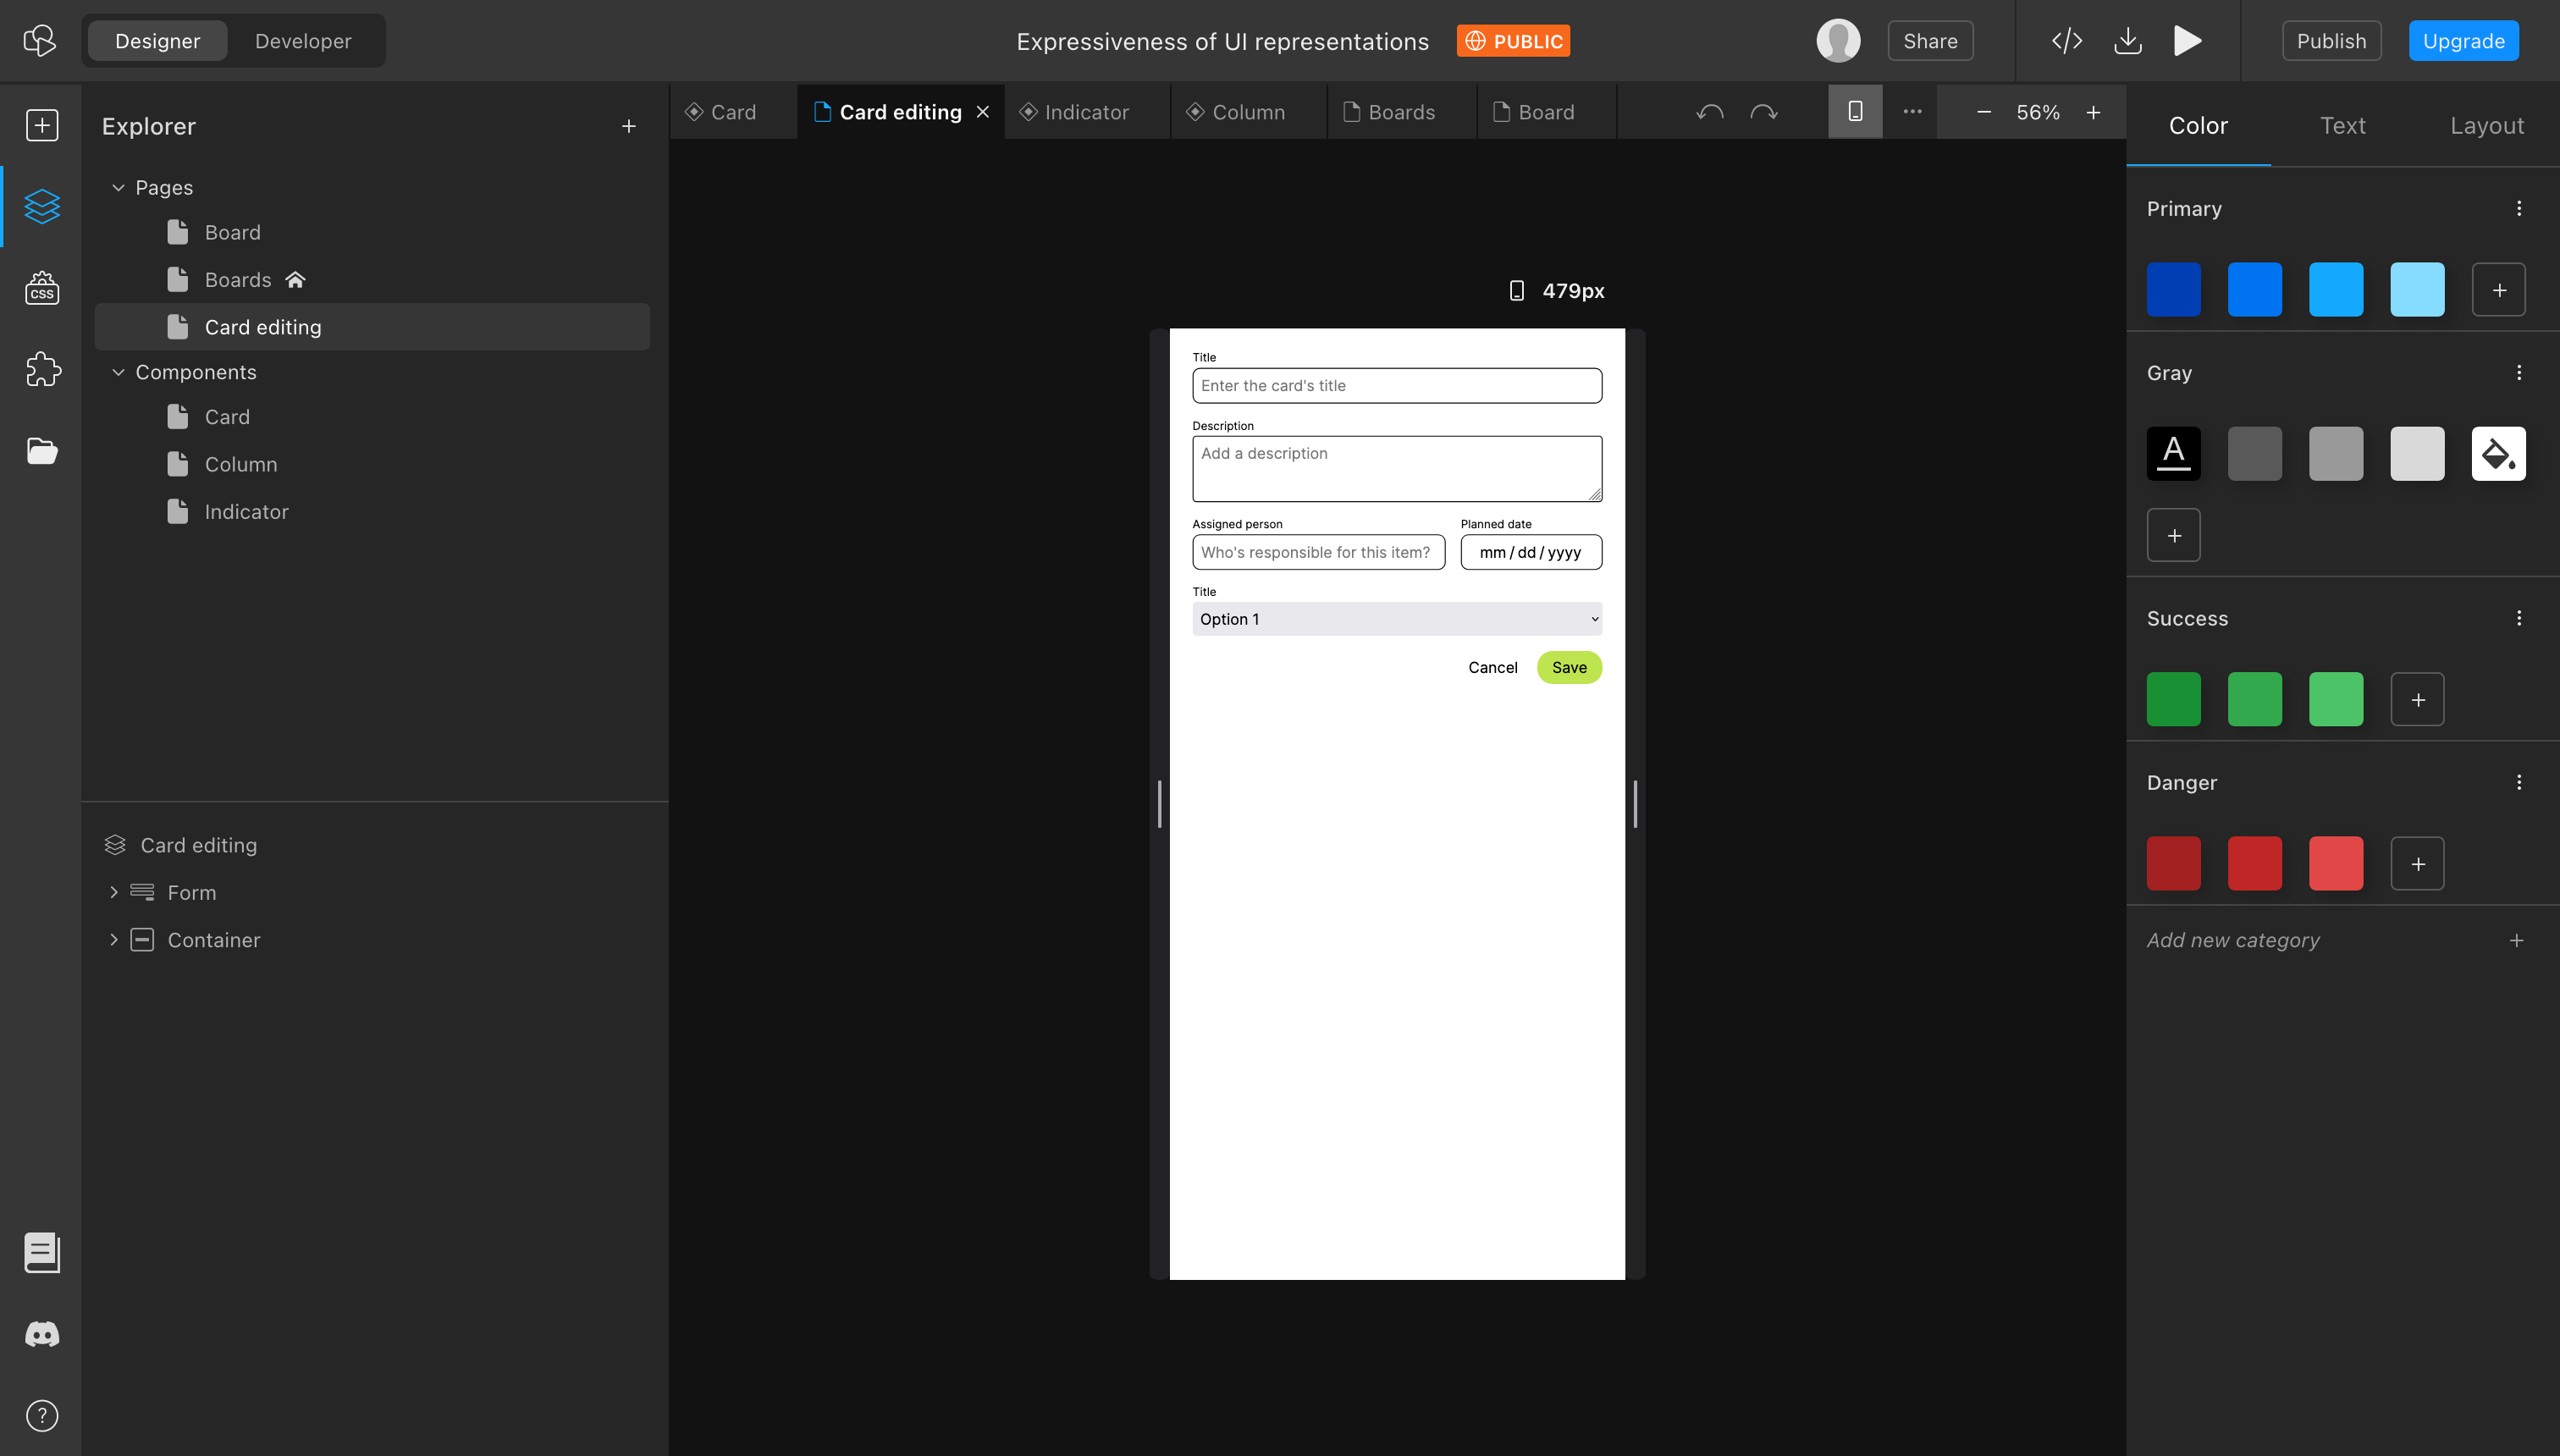
\includegraphics[width=\textwidth]{4-results-and-discussion/openuidl-editor}
    \caption{Screenshot of the OpenUIDL editor}
    \label{fig:4-2-openuidl-editor}
\end{figure}

The overall development experience using Quid could be described as passable.
The editor swiftly colored the syntax and provided simple code completion, as well as accurately previewing the described components in real-time or pointing out to errors in the language syntax.
Unfortunately, the error messages were not too descriptive on their own and the documentation for the project was too scarce to provide any helpful guidance.

The editor for OpenUIDL, even though it is a much more complex application, was easier to use.
It also did not suffer from any performance issues and practically no errors disrupted the development flow.
The only instance of unexpected behavior occurred when using slots (inputs for content), when placeholders were displayed as empty even when they were filled with content.
The interface of the application was for the most part intuitive, although sometimes editing the design was not as comfortable as expected.
The company behind the editor and the language also provides quite comprehensive support for the tool: apart from comprehensive documentation, there are also YouTube tutorials available, as well as a dedicated Discord server where it is possible to interact with the community and support team directly.

To sum up, although Quid and its editor present some noteworthy capabilities, the whole still looks like a proof of concept, and not a complete application (this is also reflected in its version).
OpenUIDL and its platform (the language, the collaborative editor, integrations, hosting and support) are much more mature in comparison; the whole solution is actually commercialized.
